% NOTE: five sentences in this section arrived truncated from the source
% document (mid-word cuts at "an oracle-informed retention policy because...",
% "Adding accelerator capacity th models...", "roughly 86% of the total problem
% disappears...", "A sta construction cost as fits...", and "The two mechanisms
% are thus that vary in practice..."). They are restored below and marked with
% % RESTORED so they can be checked against intent.

\section{Gaps, Insights and Opportunities}

\subsection{Agents Break Existing HPC DMSH Solutions}

\paragraph{Agents Create Workflow Nondeterminism.}
Although their impact on scientific goals is significant, AI-steered HPC
workflows break a fundamental assumption made by memory-storage software DSM
systems about scientific HPC workflows: that of predictable phases and data
accesses. AI steering agents make independent choices about which data will be
used for computation in an upcoming phase (and in some cases even about which
phases will be triggered). As a result, prior systems that treat storage as an
extension of memory are unable to prefetch the correct data for each step in
agentic HPC workflows because they rely on the definition of deterministic
phases in an HPC workflow program. This leads to stalls while the required
data is fetched from storage into memory. Figure~\ref{fig:predictability}
demonstrates the proportion of runs of the same workflow that deviate from the
most common action taken at a given step index. With only 30--60\% agreement
at any given step, it exemplifies that even given the exact same task to
investigate, agentic frameworks will produce significantly different behavior.
Functionally, agentic workflows are not deterministic.

\begin{figure}[t]
\centering
% PLOT SPEC (kept for provenance; rendered by
% scripts/figures/make_figures.py -> figure_drafts/fig-predictability.pdf)
%   $x$ = step index, $y$ = share of runs taking the modal action at that 
%   step, over repeated executions of an identical task. Band the 30--60\% 
%   region. Optionally overlay a second series for a second workflow to show 
%   the pattern is not workload-specific.
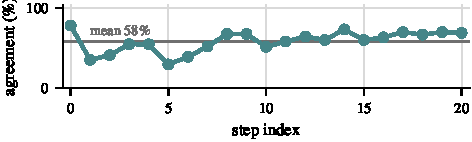
\includegraphics[width=\columnwidth]{figures/fig-predictability}
\caption{Agreement with the modal action at each step index across repeated
executions of an identical task. Agreement never exceeds 60\%, so the same
request produces materially different executions.}
\label{fig:predictability}
\end{figure}

\paragraph{Agents Add Memory Pressure.}
To make matters worse, the core problem these solutions address is compounded
in AI-steered workflows because AI agents comprise multi-billion-parameter
models requiring anything from 2--200~GB of space (for most common models).
The loading of model weights from disk all the way to GPU VRAM is some of the
most expensive loading work in a workflow, and as such agentic workflows
typically offload models that may be reused later onto CPU RAM. However, this
means models are now in competition with the scientific data they work with
for the RAM resources available, exacerbating the memory pressure HPC
workflows experience. Figure~\ref{fig:replacement-loss} shows a visual
workflow timeline against the page cache hits of a workflow over time, showing
how typical ``weight-parking'' behavior can cycle useful data out of RAM.

\begin{figure}[t]
\centering
% PLOT SPEC (kept for provenance; rendered by
% scripts/figures/make_figures.py -> figure_drafts/fig-replacement-loss.pdf)
%   two aligned panels sharing an $x$ axis of wall time. Top: workflow 
%   timeline with model-load, model-park and tool-invocation spans. Bottom: 
%   page-cache hit rate (or resident bytes) for the scientific artifact. 
%   Annotate the points where a park event is followed by a collapse in the 
%   artifact's residency and a subsequent re-read.
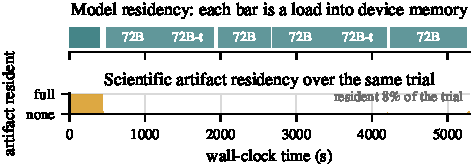
\includegraphics[width=\columnwidth]{figures/fig-replacement-loss}
\caption{Model parking evicts scientific data. Each parking event coincides
with a loss of the artifact's residency, which the next tool invocation must
pay to rebuild.}
\label{fig:replacement-loss}
\end{figure}

\paragraph{Agents Rely Heavily On Data Transformations.}
Data used by agentic tools must undergo a representation change. A
representation change is work that produces a structure the consumer could not
have obtained by placing bytes. In other words, if the in-memory structure the
consumer requires is byte-identical to some contiguous range of the
file---modulo a header---then making it usable is placement. Otherwise the
structure is a computed function of the file, and producing it is a
representation change. These representation changes are responsible for 93\%
on average of the stalls caused by waiting for data staging. Because the
product of a representation change is a computed structure rather than a range
of a file, it cannot be named, staged, or evicted by a byte-oriented tier at
all: it exists only as anonymous memory inside a live consumer process. Parked
model weights have the same property, for the same reason. The ceiling on a
placement-oriented system is therefore set by which rungs of the cost chain
its interface can reach, not by how accurately it predicts---no improvement in
prediction moves a cost the interface cannot express. And because the retained
structure and the parked model both occupy anonymous memory drawn from a
single allocation, the question these workflows pose is not which bytes to
fetch but which structures to keep, and---when they cannot all be kept---which
of them a gigabyte of memory is better spent on.

\subsection{Value-Ranking Opportunities}

\paragraph{Not Every GB Retained Is Equally Valuable.}
If retention is the action, a scheduler needs a price: how many seconds of
future stall a gigabyte of held memory buys. That price is not uniform, and it
is non-uniform in a way that rules out any fixed policy. Holding logical
content fixed---the same array, bit for bit, in six serialisations---the
seconds saved per gigabyte retained span $65\times$, from 22.0 for ASCII
numeric text to 0.34 for a memory-mappable binary layout
(Figure~\ref{fig:sgb-spread}). Model weights occupy a far narrower band of
2.78--3.81, and for a structural reason: a model's cost is dominated by moving
bytes at roughly fixed bandwidth, so it is near-linear in size and its price
per gigabyte is nearly constant. Data has no such anchor, because the cost of
a representation change is set by the decoder rather than by the byte count.

The consequence is that models land in the middle of the data range rather
than above or below it. Some artifacts are worth an order of magnitude more
per gigabyte than any model; others are worth almost nothing. A fixed class
priority---models first, or data first---is therefore wrong at one end of the
range or the other, and the correct ordering is recoverable only by pricing
each resource individually.

Two properties make that pricing practical. First, the price is a property of
the representation rather than of the instance: across a $4\times$ size range
it is flat to within 1.00--1.16$\times$, so it can be measured once per format
and reused without profiling. Second, there is a floor. Materialising any
structure into a process address space costs roughly 0.32~s/GB regardless of
format, so a resource whose price approaches that floor performs no
transformation at all, and retaining it buys nothing that placement would not.

\begin{figure}[t]
\centering
% PLOT SPEC (kept for provenance; rendered by
% scripts/figures/make_figures.py -> figure_drafts/fig-sgb-spread.pdf)
%   seconds saved per GB retained, log $y$, one point per resource. Shade 
%   the narrow model band (2.78--3.81) as a horizontal strip; scatter the 
%   data artifacts across it, from ASCII at 22.0 to memory-mappable binary 
%   at 0.34. Draw a horizontal rule at the 0.32~s/GB materialisation floor. 
%   The models-in-the-middle geometry is the reading.
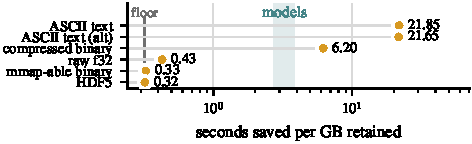
\includegraphics[width=\columnwidth]{figures/fig-sgb-spread}
\caption{Retention value per gigabyte across resources. Models occupy a narrow
band set by transfer bandwidth; data artifacts span $65\times$ and bracket
that band on both sides, so no fixed class priority is correct.}
\label{fig:sgb-spread}
\end{figure}

\paragraph{Value-Aware Retention vs.\ Prefetching Depend on Hardware Topology
and the Inter-need Gap.}
Retention and speculative staging are not two implementations of one idea;
they serve disjoint populations of stalls. Retention can only help a resource
used more than once---a first use has nothing to retain---while staging is the
only mechanism that can help a first use at all. Which dominates is therefore
set by reuse density: resource needs per distinct resource.

That quantity moves with scale. Holding schedule length fixed and growing the
resource population from 5 to 28, the share of needs that are first uses rises
from 10.4\% to 32.3\%, and the advantage shifts correspondingly from retention
toward staging (Figure~\ref{fig:scale-sweep}). The shift is structural rather
than a matter of prediction quality: an oracle-informed retention policy fades
over the same range, because the misses it could convert are progressively not
there to convert.  % RESTORED

Hardware topology moves the balance a second way, and in both directions.
Accelerator capacity and host memory are separate budgets, and a model
actively resident on an accelerator charges neither. Adding accelerator
capacity therefore removes precisely the models most worth retaining, leaving
a less-used remainder to compete for host memory and shrinking what
value-aware arbitration can recover.  % RESTORED
Host memory behaves symmetrically: once the budget is large enough that
nothing is ever evicted---in our configuration at roughly 86\% of the total
footprint---the arbitration problem disappears and retaining everything is
correct.  % RESTORED
Budget also buys value in steps rather than smoothly, since additional memory
pays only when it crosses a threshold admitting one more resource
(Figure~\ref{fig:topology-budget}).

Finally, the inter-need gap bounds what staging can achieve. A stage recovers
only as much of a construction cost as fits into the window before the need
arrives, so the same mechanism captures more as computation between tool calls
grows.  % RESTORED
Retention has no such dependence---its saving is the full construction cost
whenever the resource is next used. The two mechanisms are thus complementary
along both axes that vary in practice, which is the case for arbitrating them
jointly rather than choosing one.  % RESTORED

\begin{figure}[t]
\centering
% PLOT SPEC (kept for provenance; rendered by
% scripts/figures/make_figures.py -> figure_drafts/fig-scale-sweep.pdf)
%   $x$ = number of distinct resources (5, 10, 18, 28). Left axis: advantage 
%   over the recency-ranked baseline for retention and for staging, as two 
%   lines that cross. Right axis: first-use share, rising 10.4\% 
%   $\rightarrow$ 32.3\%. The crossing is the reading.
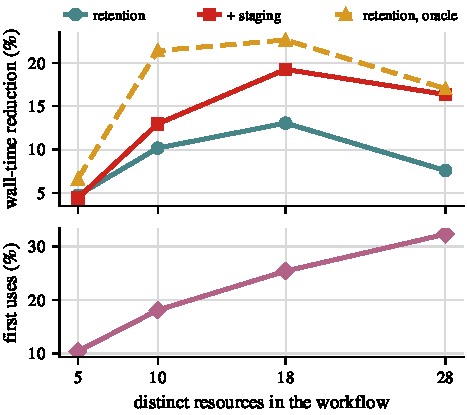
\includegraphics[width=\columnwidth]{figures/fig-scale-sweep}
\caption{As the resource population grows at fixed schedule length, first uses
become a larger share of all needs and the advantage moves from retention to
staging.}
\label{fig:scale-sweep}
\end{figure}

\begin{figure}[t]
\centering
% PLOT SPEC (kept for provenance; rendered by
% scripts/figures/make_figures.py -> figure_drafts/fig-topology-budget.pdf)
%   $x$ = budget as \% of total footprint. $y$ = share of decisions in which 
%   memory pressure forced an eviction, one line per accelerator-slot count, 
%   falling to zero. Mark the packing thresholds with vertical rules so the 
%   step structure is visible. This is the motivating view; 
%   Figure~\ref{fig:budget-sweep} shows the same axis with performance 
%   rather than pressure.
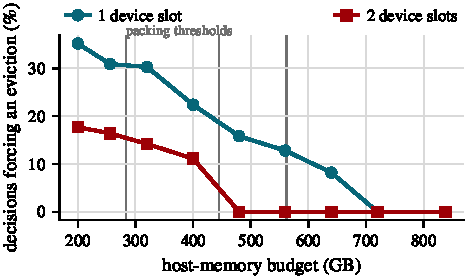
\includegraphics[width=\columnwidth]{figures/fig-topology-budget}
\caption{Contention as a function of budget and accelerator capacity. Above
roughly 86\% of the total footprint nothing is ever evicted and the
arbitration problem disappears; below it, budget admits resources in steps
rather than smoothly.}
\label{fig:topology-budget}
\end{figure}

\subsection{Speculative Value-Ranking Opportunities}

\paragraph{Local transition structure survives workflow-level nondeterminism.}
Agentic workflows are dynamic in the large but structured in the small: tools
exhibit high-confidence $k$-offset successor relationships, in which one tool
consistently follows another a fixed number of invocations later. Not every
tool has such a successor at every offset, but nearly every tool has one at
some offset. Figure~\ref{fig:tool-relationships} shows this for AtomAgents at
both framework and workflow level---restricting to $k \in [0,5]$, both
workflows contain numerous relationships with empirical confidence between 0.9
and 1.0. Critically, these relationships persist across substantially
different prompts and objectives within a framework, so traces from prior,
unrelated executions supply useful priors on the first run of a workflow never
seen before.

\paragraph{Plans predict order, not distance.}
Frameworks organised by a planner agent expose a second, longer-range signal:
a natural-language plan naming the tools to be invoked and their intended
order. In AtomAgents these plans predict 95\% of tool orderings correctly
(Figure~\ref{fig:plan-accuracy}), far enough ahead to begin staging resources
whose construction would otherwise be exposed. What they do not supply is
distance: agents insert additional calls to recover from syntax errors and
retry failures, so the observed trace diverges from the planned offsets even
when the order is right. Plans therefore reach far but locate poorly, while
local transitions locate well but do not reach---which is why the two are used
together.

\begin{figure}[t]
\centering
% PLOT SPEC (kept for provenance; rendered by
% scripts/figures/make_figures.py -> figure_drafts/fig-tool-relationships.pdf)
%   heatmap or matrix, source tool $\times$ offset $k \in [0,5]$, cell 
%   shaded by the confidence of the highest-confidence successor at that 
%   offset. Two panels: framework level and workflow level. Highlight cells 
%   in the 0.9--1.0 band. The reading is that nearly every row has at least 
%   one dark cell.
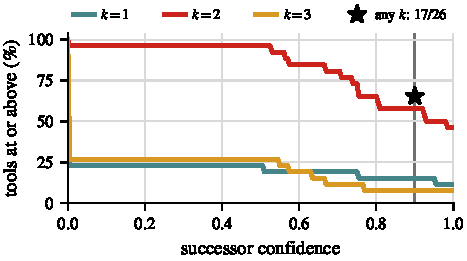
\includegraphics[width=\columnwidth]{figures/fig-tool-relationships}
\caption{High-confidence $k$-offset successor relationships in AtomAgents.
Nearly every tool has at least one successor at some offset with confidence
above 0.9, despite workflow-level nondeterminism.}
\label{fig:tool-relationships}
\end{figure}

\begin{figure}[t]
\centering
% PLOT SPEC (kept for provenance; rendered by
% scripts/figures/make_figures.py -> figure_drafts/fig-plan-accuracy.pdf)
%   planned tool order versus realized tool order. Either (a) a 
%   confusion-style plot of planned rank versus realized rank, or (b) paired 
%   bars for ordering accuracy (95\%) against offset-distance accuracy (much 
%   lower). Option (b) makes the order-vs-distance contrast, which is the 
%   point of the paragraph.
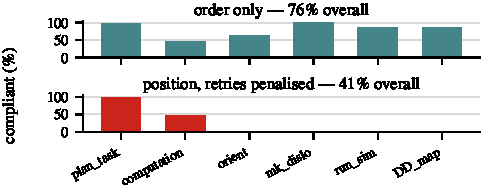
\includegraphics[width=\columnwidth]{figures/fig-plan-accuracy}
\caption{Planner-declared orderings are accurate; planner-implied distances
are not. Agents insert recovery and retry calls, so realized offsets diverge
from planned ones even when the order is correct.}
\label{fig:plan-accuracy}
\end{figure}
